\documentclass[review]{elsarticle}
\usepackage{lineno,hyperref}
\modulolinenumbers[5]
\usepackage[margin=1in]{geometry}
\usepackage{graphicx}
\usepackage{placeins}
\usepackage{comment}

\bibliographystyle{elsarticle-num}

\begin{document}
\begin{frontmatter}
\title{Evaluation of the anisotropic grain boundaries and surfaces of $\alpha$ U via molecular dynamics}

\author[ncsu]{Khadija Mahbuba}
\author[ncsu,inl]{Benjamin Beeler}
\author[inl]{Andrea Jokisaari}
\address[ncsu]{North Carolina State University, Raleigh, NC 27607}
\address[inl]{Idaho National Laboratory, Idaho Falls, ID 83415}

\begin{abstract}

Abstract text

\end{abstract}
\end{frontmatter}

\linenumbers

\section{Introduction}

Intro text


\FloatBarrier

\section{Computational Details}

comp details text. below is Fig. \ref{fig:grb_ex}. 

\begin{figure}[!htp]
\begin{center}
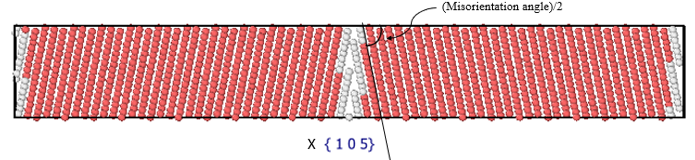
\includegraphics[width=0.6\textwidth]{Picture1}
\end{center}
\caption{Caption for this Fig.  }
\label{fig:grb_ex}
\end{figure}

\FloatBarrier

\section{Results}
\subsection{$\alpha$-U Grain Boundary Energies}
\subsubsection{Tilting of XY face of alpha U}



\subsubsection{Tilting of YZ face of alpha U}


\subsubsection{Tilting of XZ face of alpha U}






\section{Conclusions}
 Conclusions text

\section{Acknowledgement}

You can leave this for now, it will change. 

Add NEAMS ackowledgement This manuscript has been authored by Battelle Energy Alliance, LLC with
the U.S. Department of Energy. The publisher, by accepting the article for publication, acknowledges that
the U.S. Government retains a nonexclusive, paid-up, irrevocable, worldwide license to publish or reproduce
the published form of this manuscript, or allow others to do so, for U.S. Government purposes. This research
made use of the resources of the High Performance Computing Center at Idaho National Laboratory, which
is supported by the Office of Nuclear Energy of the U.S. Department of Energy and the Nuclear Science
User Facilities.




\bibliography{../MARMOTbib}


\end{document}  
